\section{Example: Relaxing the Assumption of Equal Transition Probabilities }\label{sec:dm_disc}


{\begin{framed}
Make a copy of the MCMC and model files you just made. 
Call them \cl{mcmc\_mk\_dicretized.Rev} and \cl{model\_mk\_discretized.Rev}. 
These will contain the new model parameters and models. \par 
\end{framed}}
\begin{figure}[h!]
\fbox{%
\begin{minipage}{\textwidth}\centering
% 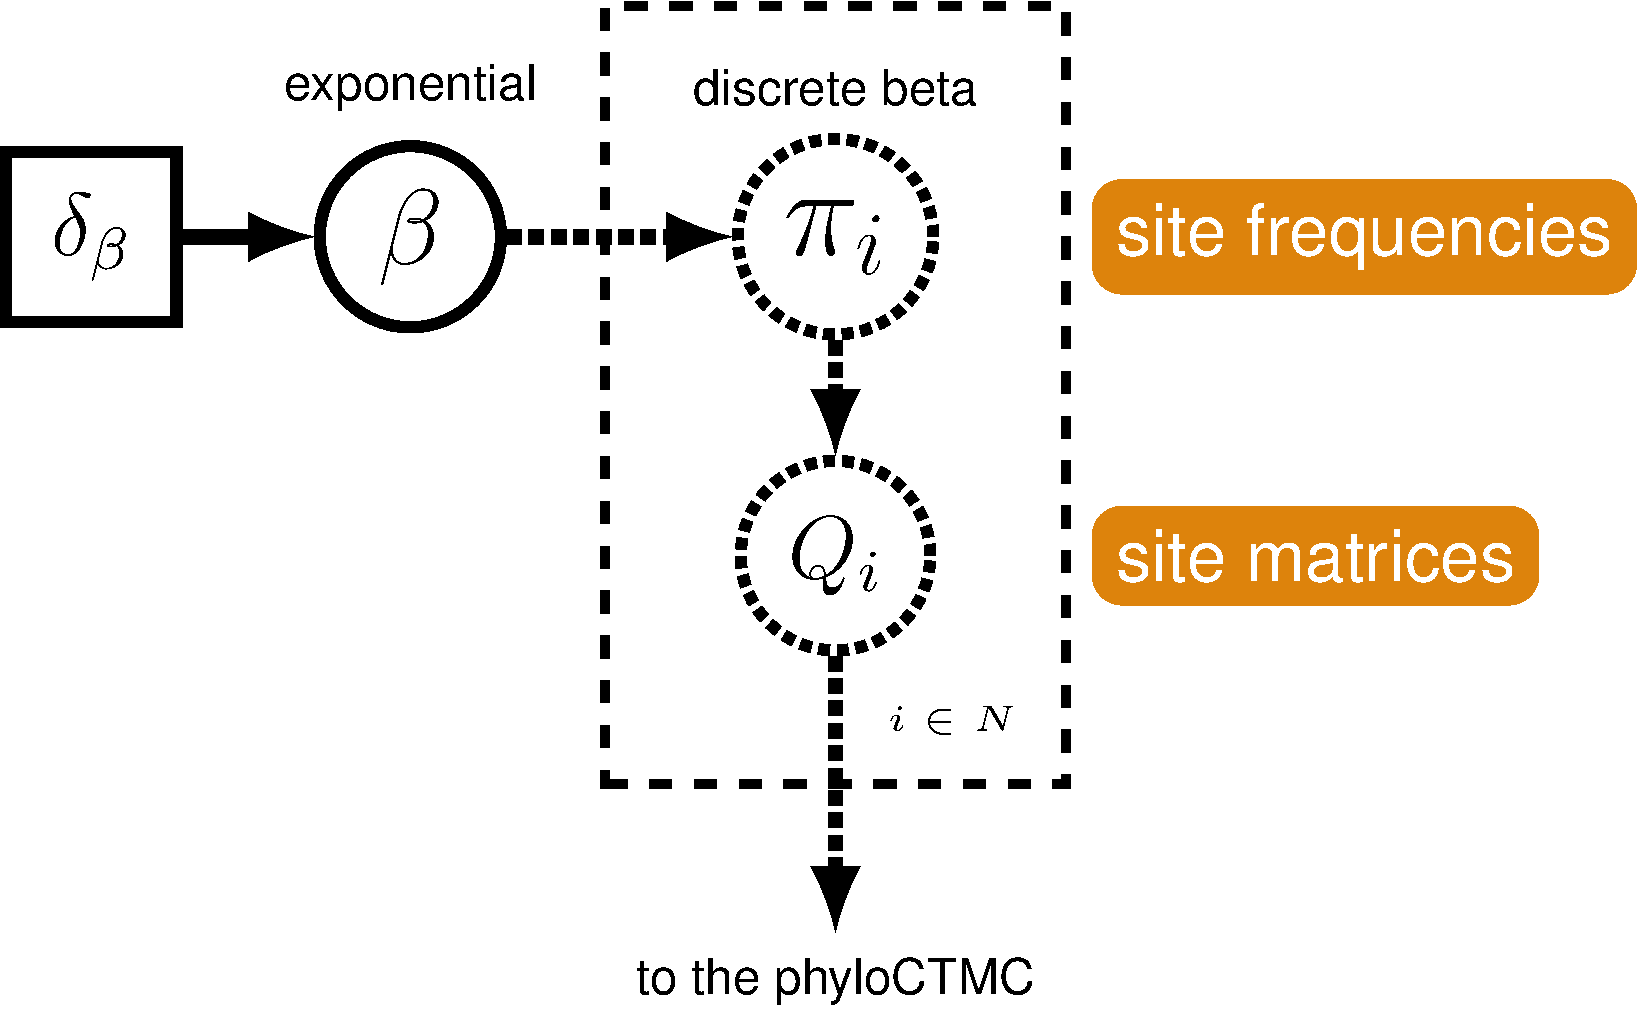
\includegraphics[width=0.5\textwidth,angle=0]{\ResourcePath figures/tikz/morpho_gm-eps-converted-to} % 
\caption{\small Graphical model demonstrating the discretized Beta distribution for allowing variable state frequencies.}
\end{minipage}}
\label{fig:module-gm}
\end{figure}
The Mk model makes a number of assumptions, but one that may strike you as unrealistic is the assumption that characters are equally likely to change from any one state to any other state.
That means that a trait is as likely to be gained as lost.
While this may hold true for some traits, we expect that it may be untrue for many others. \par
\cl{RevBayes} has functionality to allow us to relax this assumption.
We do this by specifying a Beta prior on state frequencies.
Remember from the \cl{RB\_CTMC} lesson that stationary frequencies impact how likely we are to see changes in a character.
For example, it may be very likely, in a character, to change from 0 to 1.
But if the frequency of 0 is very low, we will still seldom see this change. \par
We can exploit the relationship between state frequencies and observed changes to allow for variable Q matrices across characters (Fig. 2).
To do this, we generate a Beta distribution on state frequencies \citep{huelsenbeck01c}, and use the state frequencies from that Beta distribution to generate a series of Q-matrices to use to evaluate our data \citep{pagel04}. \par
This type of model is called a \textbf{mixture model}.
There are assumed to be subdivisions in the data, which may require different parameters (in this case, state frequencies).
These subdivisions are not defined \textit{a priori}. 
This model has previously been shown to be effective for a range of empirical and simulated datasets \citep{wright16}.\par




\subsection{Modifying the MCMC File}

At each place in which the output files are specified in the MCMC file, change the output path so you don't overwrite the output from the previous exercise. 
For example, you might call your output file \cl{output/mk\_discretized.log} and \cl{output/mk\_discretized.trees}.
Change source statement to indicate the new model file.

\subsection{Modifying the Model File}

Open the new model file that you created. We need to modify the way in which the Q matrix is specified. 
We will use a discretized Beta distribution to place a prior on state frequencies. 
The Beta distribution has two parameters, $\alpha$ and $\beta$.
These two parameters specify the shape of the distribution.
State frequencies will be evaluated according to this distribution, in the same way that rate variation is evaluated according to the Gamma distribution. 
The discretized distribution is split into multiple classes, each with it's own set of frequencies for the 0 and 1 characters.
The number of classes can vary; we have chosen 4 for tractability.\par

{\tt \begin{snugshade*}
\begin{lstlisting}
n_cats = 4
alpha_ofbeta ~ dnExponential( 1 )
beta_ofbeta ~ dnExponential( 1 )
moves[mvi++] = mvScale(alpha_ofbeta, lambda=1,    weight=1.0 )
moves[mvi++] = mvScale(alpha_ofbeta, lambda=0.1,  weight=3.0 )
moves[mvi++] = mvScale(alpha_ofbeta, lambda=0.01, weight=5.0 )
moves[mvi++] = mvScale(beta_ofbeta, lambda=1,    weight=1.0 )
moves[mvi++] = mvScale(beta_ofbeta, lambda=0.1,  weight=3.0 )
moves[mvi++] = mvScale(beta_ofbeta, lambda=0.01, weight=5.0 )
\end{lstlisting}
\end{snugshade*}}

Above, we initialized the number of categories,  the parameters to the Beta distribution, and the moves on the parameters to the Beta. 

Next, we set the categories to each represent a quadrant of the Beta distribution specified by the \cl{alpha\_ofbeta} and \cl{beta\_ofbeta}. The {\tt +1} values are added to the beta shape and scale parameters to prevent model overfitting.

{\tt \begin{snugshade*}
\begin{lstlisting}
cats := fnDiscretizeBeta(alpha_ofbeta+1, beta_ofbeta+1, 4)
\end{lstlisting}
\end{snugshade*}}

If you were to print the \cl{cats} variable, you would see a list of state frequencies like so:

{\tiny{\tt \begin{snugshade*}
\begin{lstlisting}
|*   0.0780943
|*   0.40457
|*   0.769453
|*   0.97106
\end{lstlisting}
\end{snugshade*}}}

Using these state frequencies, we will generate a new vector of Q matrices.
Because we are varying the state frequencies, we must use a Q matrix generation function that allows for state frequencies to vary as a parameter.
We will, therefore, use the \cl{fnF81} function.

{\tt \begin{snugshade*}
\begin{lstlisting}
for (i in 1:cats.size())
{
    Q[i] := fnF81(simplex(abs(1-cats[i]), cats[i]))
}
\end{lstlisting}
\end{snugshade*}}

Once we've made the our vector of matrices, we specified moves on our matrix vector:
{\tt \begin{snugshade*}
\begin{lstlisting}
matrix_probs ~ dnDirichlet(v(1,1,1,1))
moves[mvi++] = mvSimplexElementScale(matrix_probs, alpha=10, weight=1.0) 
\end{lstlisting}
\end{snugshade*}}

This Dirichlet prior says that no category is expected to have more characters than another. If you expected some category to hold more of the characters, you could put more weight on that category. \par

The only other specification that needs to change in the model file is the CTMC:
{\tt \begin{snugshade*}
\begin{lstlisting}
phyMorpho ~ dnPhyloCTMC(tree=phylogeny, siteRates=rates_morpho, Q=Q, type="Standard", coding="variable", siteMatrices=matrix_probs)
\end{lstlisting}
\end{snugshade*}}

You'll notice that we've added a command to tell the CTMC that we have multiple site matrices that will be applied to different characters in the matrix.

\medskip
\subsubsection{Set-Up the MCMC}

The MCMC chain set-up does not need to change. 
Run the new MCMC file, just as you ran the plain Mk file.
This estimation will take longer than the Mk model, due to increased model complexity. \par


\section{Site-Heterogeneous Discrete Morphology Model} \label{sec:dm_dir}

\begin{figure}[h!]
\fbox{%
\begin{minipage}{\textwidth}\centering
\includegraphics[width=0.5\textwidth,angle=0]{\ResourcePath figures/catplate}
\caption{\small Graphical model demonstrating the Dirichlet prior to allow variable state frequencies in both binary and multistate data.}
\end{minipage}}
\label{fig:module-relaxed morphology}
\end{figure}

In the previous example, we explored allowing among-character variation in state frequencies.
This is an excellent start for allowing more complex models for morphology.
But this approach also has several shortcomings.
First, because we use a Beta distribution, this model really only works for binary data.
Secondly, oftentimes, we will not have a good idea of the shape of the distribution from which we expect state frequencies to be drawn. \par
To accommodate for these concerns, \cl{RevBayes} also has a model that is similar to the CAT model \citep{lartillot04}. \par
The site-heterogeneous discrete morphology model (SHDM) uses a hyperprior on the prior on state frequencies to mix over different possible combinations state frequencies.
In this mixture model, F81 Q-matrices (an extension of the Jukes-Cantor which allows for different state frequencies between characters) is initialized from a set of state frequencies.
The number of Q-matrices initialized is equal to the number of user-defined categories, as in the discretized Beta model.
The state frequencies used to initialize the Q-matrices are drawn from a Dirichelet prior distribution, which is generated by drawing values from an exponential hyperprior distribution. 
This model is visualized in Fig. 3.\par

\subsection{Example: Site-Heterogeneous Discrete Morphology Model }

{\begin{framed}
Make a copy of the MCMC and model files you just made. 
Call them \cl{mcmc\_mk\_hyperprior.Rev} and \cl{model\_mk\_hyperprior.Rev}. 
These will contain the new model parameters and models. \par 
\end{framed}}

\subsection{Modifying the MCMC File}

At each place in which the output files are specified in the MCMC file, change the output path so you don't overwrite the output from the previous exercise. 
For example, you might call your output file \cl{output/mk\_hyperprior.log} and \cl{output/mk\_hyperprior.trees}.
We will also monitor Q\_morpho and pi.
Add Q\_morpho and pi to the \cl{mnScreen}. 
Change source statement to indicate the new model file.

\subsection{Modifying the Model File}
Open the new model file that you created. We need to modify the way in which the Q-matrix is specified.
First, we will create a hyperprior called \cl{dir\_alpha} and specify a move on it.
{\tt \begin{snugshade*}
\begin{lstlisting}
dir_alpha ~ dnExponential(1)
moves[mvi++] = mvScale(dir_alpha, lambda=1,    weight=1.0 )
moves[mvi++] = mvScale(dir_alpha, lambda=0.1,  weight=3.0 )
moves[mvi++] = mvScale(dir_alpha, lambda=0.01, weight=5.0 )
\end{lstlisting}
\end{snugshade*}}

This hyperparameter, dir\_alpha, will be used as a parameter to a Dirichelet distribution from which our state frequencies will be drawn.

{\tt \begin{snugshade*}
\begin{lstlisting}
pi_prior := v(dir_alpha,dir_alpha)
\end{lstlisting}
\end{snugshade*}}

If you were using multistate data, the dir\_alpha can be repeated for each state.
Next, we will modify our previous loop to use these state frequencies to initialize our Q-matrices.

{\tt \begin{snugshade*}
\begin{lstlisting}for(i in 1:n_cats)
{
	pi[i] ~ dnDirichlet(pi_prior)
    moves[mvi++] = mvSimplexElementScale(pi[i], alpha=10, weight=1.0) 
    
    Q_morpho[i] := fnF81(pi[i])
}
\end{lstlisting}
\end{snugshade*}}

In the above loop, for each of our categories, we make a new draw of state frequencies from our Dirichelet distribution (the shape of which is determined by our dir\_alpha values).  
We then use \cl{fnF81} to make our Q-matrices.
For each \cl{RevBayes} iteration, we will have 4 pi values and 4 Q-matrices, one for each of the number of categories we specified. \par

No other aspects of the model file need to change.
Run the MCMC as before. \par
